\section{Background}
\subsection*{Pharmacokinetic Modelling}

Broadly, pharmacokinetics is the study of the dynamics of a mass of drug in the body and is concerned with the absorption, distribution, metabolism, and excretion of that drug.  Differential equations (equations which relate the derivative of an unknown function to itself) are often used to describe how these dynamics evolve over time. The differential equation models in pharmacokinetics are called “compartmental models” as they idealize different parts of the body as compartments from which drug can flow in and out at rates proportional to how much drug is presently in that compartment. If the differential equation is not too complex, the solution can be written in terms of analytic functions.  In the case where the differential equation can not be solved in terms of analytic functions, a rich literature of numerical techniques exist to approximate the solution to within quantifiable precision. In either case, estimation of model parameters is of  interest as they represent pharmacokinetic measures, such as the volume of distribution or rate constants for which the drug is absorbed into/excreted out of a compartment. If the parameters for such a model are known, we can use the models to make predictions about drug concentration as a function of time and dose. This in turn can be used to select a dose that meets given criteria about what the concentration function should look like.

Parameter estimation for these models can be done in both frequentist and Bayesian frameworks.  In a Bayesian framework, parameter estimation begins by specifying a prior distribution which reflects the knowledge of parameters before seeing data. Once data are observed, Bayes’ rule can be used to get the posterior distribution.  This distribution provides information about what parameter values have most plausibly generated the observed data.  By virtue of being a probability distribution, the posterior can be summarized by expectations to get point estimates of model parameters. Shown in \cref{fig:fig1} is a visual summary of how Bayes’ rule and Bayesian modelling of pharmacokinetics works using pseudodata. The leftmost panel is our prior distribution.  Each concentration curve results from specific combinations of parameters for the model which are believed to be plausible before seeing data.  Once data are observed (the middle panel), application of Bayes’ rule yields the rightmost panel.  Concentration curves in this panel correspond to combinations of parameters which have most plausibly generated the data, resulting in concentration curves which have most plausibly generated the data. Note that in this setting, because we have many measurements, the pharmacokinetic model is well-determined and the posterior uncertainty is small. Except in very simple cases, the integrals required to evaluate the posterior quickly become intractable, thus computational approximations are required to fit Bayesian models.
%
\begin{figure} [h!]
	\centering
	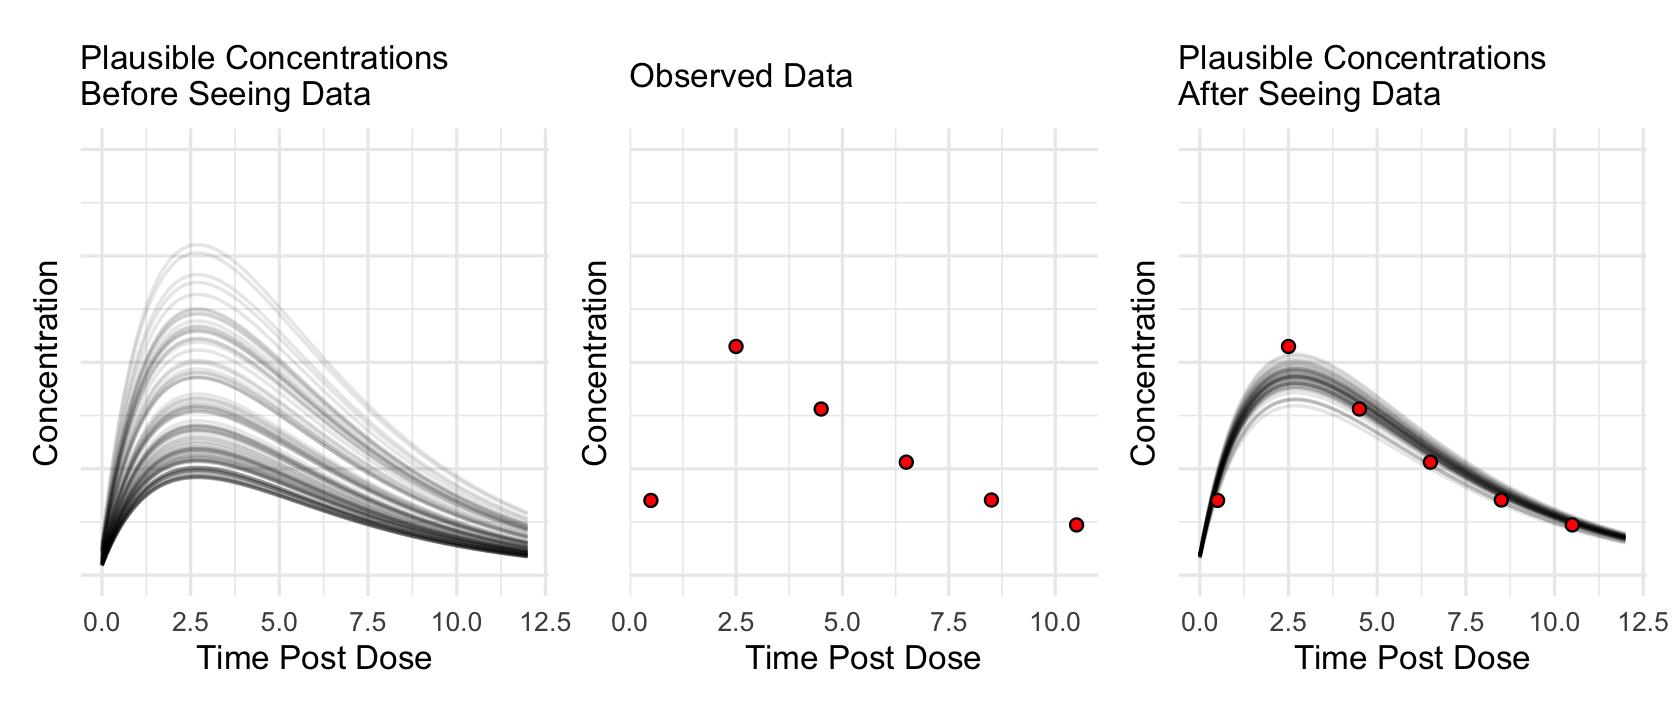
\includegraphics[width=\linewidth]{figs/fig_1}
	\caption{A demonstration of a Bayesian workflow for pharmacokientic models.  The leftmost panel represents the prior.  Each curve corresponds to a unique set of model parameters which induce each concentration function.  In the center panel is the data observed from a single patient.  Conditioning on this data yields the rightmost panel.  Each curve corresponds to a unique set of model parameters drawn from the posterior distribution.} 
	\label{fig:fig1}
\end{figure}
%
\subsection*{Dosing Decisions}

Vitamin K antagonists, such as the popular oral anticoagulant Warfarin, are known to have narrow therapeutic windows as well as drug and food interaction. Determination of a maintenance dose is consequently a procedure with frequent monitoring and followup, with some sources recommending monitoring daily or every other day until the INR stabilizes for two days.  The narrow therapeutic window forces investigators to also consider the pharmacodynamics (the study of the onset, intensity, and duration of the drug response and how these are related to the concentration of the drug at its site of action) of Warfarin in addition with the pharmacokinetics when determining dose size as concentration of the drug alone is not sufficient to infer the antithrombotic effect in patients. The introduction of factor Xa inhibitors like apixaban has alleviated some of the difficulties in prescribing anticoagulants.  Factor Xa inhibitors have been shown to have lower risk for bleeding than Warfarin in patients with atrial fibrillation \cite{vinogradova2018risks} and also allow for fixed dosing without frequent monitoring INR. Furthermore, unlike Warfarin, the pharmacodynamic effect of apixaban on clotting is closely correlated with the concentration in the plasma \cite{Byon2019-gf}, making pharmacokinetic modelling more informative on antithrombotic effect as compared to Warfarin.  However, as of writing this paper there is little information on the therapeutic window, making selecting dose sizes large enough to avoid thromboembolism difficult. Furthermore, studies have demonstrated that inter-patient variability of apixaban plasma concentrations is much higher than was initially believed {\bf CITE MARKUS}. In this work, we develop personalized dosing whose goal is to find the minimum dose that avoids plasma concentrations that are too low. 

